\documentclass[UTF8]{ctexart}
%%%%%%%%%%%%%%%%%%%%%%%%%%%== 引入宏 ==%%%%%%%%%%%%%%%%%%%%%%%%%%%%%
\usepackage{cite}
\usepackage{amsmath}	% 使用数学公式
\usepackage{graphicx}	% 插入图片/PDF/EPS 等图像
\usepackage{subfigure}	% 使用子图像或者子表格
\usepackage{geometry}	% 设置页边距
\usepackage{fancyhdr}	% 设置页眉页脚
\usepackage{setspace}	% 设置行间距
\usepackage{hyperref}	% 让生成的文章目录有链接,点击时会自动跳转到该章节
\usepackage{url}
\usepackage{caption2}
\usepackage{listings}
\usepackage{xcolor}

\lstset{
 columns=fixed,
 numbers=left,                                        % 在左侧显示行号
 numberstyle=\tiny\color{gray},                       % 设定行号格式
 frame=none,                                          % 不显示背景边框
 backgroundcolor=\color[RGB]{245,245,244},            % 设定背景颜色
 keywordstyle=\color[RGB]{40,40,255},                 % 设定关键字颜色
 numberstyle=\footnotesize\color{darkgray},
 commentstyle=\it\color[RGB]{0,96,96},                % 设置代码注释的格式
 stringstyle=\rmfamily\slshape\color[RGB]{128,0,0},   % 设置字符串格式
 showstringspaces=false,                              % 不显示字符串中的空格
 language=c,                                        % 设置语言
}


%%%%%%%%%%%%%%%%%%%%%%%%%%== 设置全局环境 ==%%%%%%%%%%%%%%%%%%%%%%%%%%%%
% [geometry] 设置页边距
\geometry{top=2.6cm, bottom=2.6cm, left=2.45cm, right=2.45cm, headsep=0.4cm, foot=1.12cm}
% 设置行间距为 1.5 倍行距
\onehalfspacing
% 设置页眉页脚
\pagestyle{fancy}
%\lhead{左头标}
%\chead{\today}
%\rhead{152xxxxxxxx}
\lfoot{}
\cfoot{\thepage}
\rfoot{}
%\renewcommand{\headrulewidth}{0.4pt}
%\renewcommand{\headwidth}{\textwidth}
%\renewcommand{\footrulewidth}{0pt}

%%%%%%%%%%%%%%%%%%%%%%%%%%== 自定义命令  ==%%%%%%%%%%%%%%%%%%%%%%%%%%%%%%
% 此行使文献引用以上标形式显示
\newcommand{\supercite}[1]{\textsuperscript{\cite{#1}}}
% 此行使section中的图、表、公式编号以A-B的形式显示

% 此行使图注、表注与编号之间的分隔符缺省,默认是冒号:
\renewcommand{\captionlabeldelim}{~}

%===================================== 标题设置  ==========================================
% \heiti \kaishu 为字体设置,ctex 会自动根据操作系统加载字体
\author{\small{\kaishu 71118415 叶宏庭}\\[2pt]
\small{\kaishu 东南大学软件学院}\\[2pt]
\small{Email:}
\url{213182964@seu.edu.cn}
}
\title{\Huge{\heiti TCP并发程序设计和C/S结构程序的开发}}
\CTEXoptions[today=old]
\date{\today} % 去除默认日期
%\date{\today}

%===================================== 正文区域  ==========================================
\begin{document}
\maketitle
% \tableofcontents % 目录内容z,注释取消掉可实现目录

\section{实验目的}{掌握TCP并发程序设计和C/S结构程序的开发,具体来说就是针对date程序,实现多进程版的并发程序,完成同样的date程序功能。}

\section{实验环境}
\subsection{操作系统:}{Ubuntu 20.04}
\subsection{辅助软件:}{CTEX(用于编写tex报告)}
\section{实验内容}
\subsection{阅读date源程序:}{在进行修改前,先完整阅读date源程序,了解socket的工作原理,通信机制。(详细代码请见附带code文件夹)}
\subsubsection{客户端程序 datetimec.c}
\text{指定服务器的地址与端口号:}
\begin{lstlisting}
memset( &servaddr , 0 , sizeof( servaddr ) );
servaddr.sin_family = AF_INET;
servaddr.sin_port = htons( 13 );

\end{lstlisting}

\text{与服务器建立连接:}
\begin{lstlisting}
if( connect( sockfd , (struct sockaddr *)&servaddr , sizeof( servaddr ) ) < 0 )  {
	printf( "connect error\n" );
	exit( 1 );
}
\end{lstlisting}

\text{读取服务器发来的内容:}
\begin{lstlisting}
while( ( n = read( sockfd , recvline , MAXLINE ) ) > 0 )  {
		recvline[ n ] = 0;
		if( fputs( recvline , stdout ) == EOF ) {
			printf( "fputs error\n" );
			exit( 1 );
		}
	}
\end{lstlisting}

\subsubsection{服务端程序 datetimes.c}
\text{监听指定端口:}
\begin{lstlisting}
servaddr.sin_family = AF_INET;
servaddr.sin_addr.s_addr = htonl( INADDR_ANY );
servaddr.sin_port = htons( 13 );

bind( listenfd , (struct sockaddr *)&servaddr , sizeof( servaddr ) );
listen( listenfd , 1024 );
\end{lstlisting}

\text{处理客户端请求:}
\begin{lstlisting}
for( ; ; )
{
    connfd = accept( listenfd , (struct sockaddr *)NULL , NULL );
    ticks = time( NULL );
    snprintf( buff , sizeof( buff ) , "%.24s\r\n" , ctime( &ticks ) );
    write( connfd , buff , strlen( buff ) );
    close( connfd );
}

\end{lstlisting}


\section{实验结果与分析}
\subsection{修改后的并发程序:}{修改后的date程序,完成多并发要求。(详细代码请见附带code文件夹)}
\subsubsection{客户端程序:}{因为并发是针对服务端的设计,所以客户端程序无需修改。}
\subsubsection{服务端程序:}{服务端程序为了实现多并发的要求,所以采用fork()函数来完成具体设计。只需修改原有的处理请求部分代码,其余部分无需修改。}
\par\text{fork函数使用:}
\begin{lstlisting}
for( ; ; )
{
    connfd = accept( listenfd , (struct sockaddr *)NULL , NULL );
    if((pid = fork()) == 0){
    	close(listenfd);
    	time_t ticks;
    	time(&ticks );
    	snprintf( buff , sizeof( buff ) , "%.24s\r\n" , ctime(&ticks) );
    	printf("%s\n", buff);
    	write( connfd , buff , strlen( buff ) );
    	close( connfd );
    	printf("%s\n", "Into sleep!!");
    	sleep(2);
    	printf("%s\n", "Out sleep and exit!!");
    	exit(0);
    }
    close(connfd);
}
\end{lstlisting}\par{首先采用fork()函数调用,来创建子进程完成请求的处理任务,在子进程中关闭监听,获取服务器的系统时间,采用write()函数完成系统时间的网络传输。}\par{为了体现本程序的并发性,这里采用了sleep() 函数来实现并发的可视化。在一个进程结束任务处理后,我们让进程休眠2s后再退出,再加上两句printf 的输出,我们就能明显看到并发程序的运行效果。(如下图所示)}\par
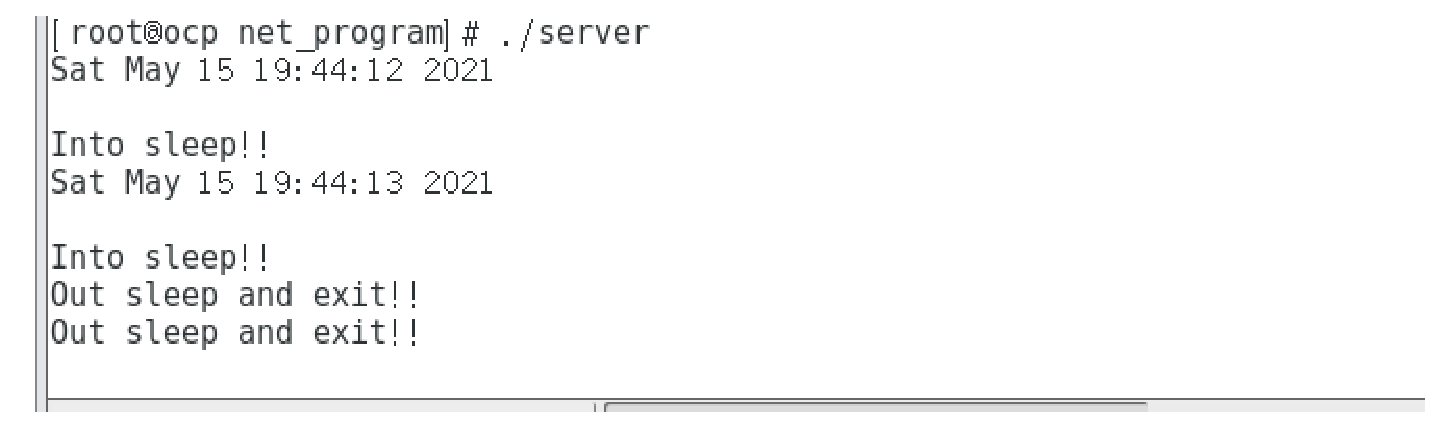
\includegraphics[scale=0.6]{result}\par{从输出的结果中我们可以看出,在第一个进程还在sleep中时,已经有别的进程为第二个用户处理了请求,最两个进程也是先后从sleep状态中醒来并且退出。}\par{从结果中,我们可以看出,这个程序完整的实现了TCP的并发设计。}
\subsection{总结}
\par{通过本次实验,初步了解了基于TCP的C/S结构程序设计,并且实现了并发的需求,改进了datetime程序,使其更加完善。}
\end{document}